\subsection{Sequentielle Modelle}
\label{sec:Kap-2.2.1}

\vspace{\baselineskip} %%% für Druck

\sttpLeserfuehrung{Bilder/Kapitel-2/Leserfuehrung/vorgehensmodelle_sequentiell_illustration.pdf}{Bilder/Kapitel-2/Leserfuehrung/vorgehensmodelle_sequentiell.pdf}

\sttpHervorhebung{\textbf{Sequentielle Vorgehensmodelle}}
\marginline{Entwicklungs\-prozess}
\sttpHervorhebung{\textbf{unterteilen die Softwareentwicklung in aufeinanderfolgende zeitliche Abschnitte (Phasen)}}. 
Dafür werden zunächst die Tätigkeiten, die zur Entwicklung eines auslieferbaren Softwareprodukts notwendig sind, zu Prozessen zusammengefasst (\zb Prozess der Anforderungsanalyse, Prozess der Implementierung). Jedem Prozess entspricht dann eine Phase des sequen\-tiel\-len Vorgehensmodells. Es wird festgelegt, in welcher Reihenfolge die Phasen nacheinander durchlaufen werden. Zudem werden für jede Phase Start- und Endpunkt geplant, die zu erreichenden Ergebnisse definiert, die auszuführenden Tätigkeiten zur Erreichung dieser Ergebnisse spezifiziert, notwendige Input- und Output-Dokumente bestimmt sowie die durchzuführenden Qualitätssicherungs- und Controllingmaßnahmen festgelegt. 

Sequentielle Vorgehensmodelle sehen eine starke Aufgabenteilung vor. So sind einige Mitarbeiter für die Planung des Softwareentwicklungsprojekts, andere für die Implementierung und wieder andere für das Testen des fertigen Softwareprodukts zuständig. Die in einer Phase als Ergebnis produzierten Artefakte werden somit häufig von \textbf{anderen} Mitarbeitern in folgenden Phasen weiterverarbeitet. Sie müssen dementsprechend vollständig und verständlich sein. Eine Phase in einem sequen\-tiel\-len Vorgehensmodell kann erst beginnen, wenn die vorhergehende Phase komplett abgeschlossen wurde, was in der Regel durch das Erreichen von zuvor definierten Meilensteinen ausgedrückt wird. In einem ideal ablaufenden Projekt ist die Kontrolle des Projektfortschritts durch die im Vorfeld terminierten Meilensteine sehr einfach. 

\vspace{\baselineskip} %%% für Druck

\sttpDefinitionskasten{\sttpDefinitionskastenSkalierungsfaktor}{Meilenstein}{Ein überprüfbares Zwischenziel innerhalb eines Projekts.}{Meilensteine werden zu Beginn eines Projekts definiert und zeitlich festgelegt. Im Laufe des Projekts kann anhand der erreichten und noch nicht erreichten Meilensteine der Projektfortschritt und der ggf. bestehende Zeitverzug im Projekt bestimmt werden. Der Begriff Meilenstein stammt aus dem klassischen Projektmanagement.}

\vspace{\baselineskip} %%% für Druck

Die strenge Form des sequentiellen Vorgehensmodells sieht vor, dass jede Phase nur genau einmal durchlaufen wird, die Phasen überschneidungsfrei sind und dementsprechend auch niemals in eine bereits abgeschlossene Phase zurückgekehrt werden kann. Dem liegt die idealisierte Vorstellung zugrunde, dass jede Phase fehlerfrei abgearbeitet werden kann und auf dieser optimalen Basis dann die folgende Phase beginnen kann. In der Praxis trifft das selten zu. Die Vorgabe, jede Phase nur einmal zu durchlaufen, würde zum Beispiel bedeuten, auch dann nicht in eine Entwurfs\-phase zurückkehren zu können, wenn Fehler oder Unvollständigkeiten des Entwurfs erst während der Implementierung auffallen. Man müsste auf Grundlage des fehlerhaften oder unvollständigen Entwurfs weiterarbeiten – wodurch das entstehende Softwareprodukt nicht (alles) das tut, was es tun soll –, oder bei der Implementierung ganz bewusst vom vorliegenden Entwurf abweichen. Letzteres würde implizit Entwurfsaktivitäten in die Phase der Implementierung verlagern, was dem Charakter eines sequentiellen Vorgehensmodells widerspricht, weil es das Konzept der inhaltlich abgegrenzten Phasen unterläuft. Die in der Praxis eingesetzten sequen\-tiel\-len Vorgehensmodelle sehen fast immer iterative Elemente vor. So kann zumindest in die zuvor abgeschlossene Phase zurückgekehrt werden, sofern Fehler, Unvollständigkeiten oder Unklarheiten bestehen. Die entsprechende Phase wird somit erneut durchlaufen und die Ergebnisse der Phase werden entsprechend angepasst. Abbildung~\ref{fig:prozesse_softwareengineering_sequentiell} zeigt Prozesse des Softwareengineering in einer sequentiellen Abfolge.

\begin{figure}[h!]
    \centering
		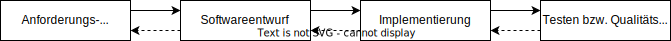
\includegraphics[width=1.0\textwidth]{Bilder/Kapitel-2/Abb-2-3.pdf}
    \caption[Prozesse des Softwareengineering in sequentieller Abfolge]{Prozesse des Softwareengineering in der sequentiellen Abfolge Anforderungsermittlung-Entwurf-Implementierung-Testen. Die gestrichelten Pfeile stellen die Rückkehrmöglichkeiten in die jeweils vorhergehende Phase dar.}
    \label{fig:prozesse_softwareengineering_sequentiell}
\end{figure}

\sttpHervorhebung{\textbf{Sequentielle Vorgehensmodelle}} 
\marginline{Umgang mit Anforderungen} 
\sttpHervorhebung{\textbf{definieren sämtliche Anforderungen zu Projektbeginn.}}
Dieser Katalog an Anforderungen bildet bei Auftragsarbeiten in der Regel auch die inhaltliche Grundlage für den Vertragsabschluss zwischen dem Auftraggeber und der Firma oder Institution, die die Softwareentwicklung übernimmt. Änderungen und Ergänzungen in Bezug auf die Anforderungen sind überhaupt nur dann möglich, wenn im Vorfeld zwischen Auftraggeber und Auftragnehmer (rechtlich) eindeutige Änderungsprozesse – vor allem in Bezug auf die Kostenübernahme – definiert wurden. Die sequentiellen Modelle eignen sich daher am besten für Projekte, deren Anforderungen von Anfang an vollständig und präzise definiert sind und in denen die Anforderungen auch über die Projektlaufzeit stabil bleiben. Implizit setzen sequentielle Vorgehensmodelle zudem voraus, dass das Softwareentwicklungsteam über einen erfahrenen Projektleiter verfügt, der anhand der Anforderungen eine realistische Abschätzung bezüglich Zeitaufwand und Kosten der Entwicklung vornehmen kann.

\sttpDefinitionskasten{\sttpDefinitionskastenSkalierungsfaktor}{Projektleiter}{Diejenige Rolle, die für ein konkretes Softwareentwicklungsprojekt organisatorische und koordinierende Aufgaben übernimmt.}{Wir verwenden den Begriff in einem sehr weiten Sinne. Die Person, die die Rolle Projektleiter übernimmt, kann gleichzeitig Personalführungsverantwortlichkeiten besitzen oder selber auch Entwicklungstätigkeiten ausführen oder mehrere Projekte leiten etc. Je nach Unternehmen bzw. Vorgehensmodell kann diese Rolle auch die Bezeichnung Projektmanager, Entwicklungsleiter, Scrum Master etc. tragen.}

\sttpHervorhebung{\textbf{Sequentielle Vorgehensmodelle}} 
\marginline{Einbezug Kunde}
\sttpHervorhebung{\textbf{binden Auftraggeber oder zukünftige Nutzer eher weniger ein.}} 
Auftraggeber und zukünftige Nutzer des Softwareprodukts werden nur zu Beginn des Projekts in den Prozess der Anforderungsermittlung einbezogen. Alle späteren Entwurfs- und Implementierungstätigkeiten sowie auch ein großer Teil der Test\-akti\-vitäten finden nur innerhalb des Entwicklungsteams statt. Dem Auftraggeber wird das Produkt erst am Ende des Projekts zur sogenannten Abnahme – Prüfung, ob das Produkt die vertraglich vereinbarte Leistung erbringt – wieder vorgelegt.

\sttpHervorhebung{\textbf{Sequentielle Vorgehensmodelle}}
\marginline{Artefakte}
\sttpHervorhebung{\textbf{sind dokumentenorientiert.}}
Als Ergebnis einer Phase entstehen ein oder mehrere Dokumente (\zb Pflichtenheft, Entwurfs\-spezifikation, Diagramm der Systemmodule), die Grundlage der nächsten Phase sind und dort weiter verfeinert, ergänzt oder angepasst werden. Eine große Heraus\-forderung besteht darin, diese Dokumente untereinander, aber auch in Bezug auf den endgültigen Programmcode des Softwareprodukts, während des gesamten Entwicklungsprozesses konsistent zu halten.
%\sttpgls{Konsistenz}

\sttpHervorhebung{\textbf{Sequentielle Vorgehensmodelle}} 
\marginline{Auslieferung}
\sttpHervorhebung{\textbf{liefern das Produkt erst mit Ende des Softwareentwicklungsprojekts aus.}} 
Zwar können auch während des Entwicklungsprozesses bereits lauffähige Versionen mit Teilfunktionalität existieren, doch werden diese nicht für den produktiven Einsatz herausgegeben.

Ein bekannter Vertreter sequentieller Vorgehensmodelle ist das Wasserfallmodell. Es ist das erste Vorgehensmodell, das in großem Maße im Softwareengineering eingesetzt wurde.
